\section{Project structure}

The main goal is to implement the methods mentioned above and to explore their results on MNIST data set, which is a simpler version of handwritten text data set. The idea is to see the qualitative results on a simple use case.
I would expect this part to work flawlessly - the results should give a se....

Next, ScrabbleGAN model will be implemented, and the methods will be adjusted to fit this use case. The results of these methods will be explored on the handwriting generation task. Will the results in this case also be  meaningful? If not, why is that and what can be improved? Are the reasons for failure inherent to the method, or is it the implementation details that should be taken more carefully?

\section{Performances and Measurements}

The tricky part of explainability is the struggle to define a good explanation. It depends on the use of the explanation. Does it have to be human interpertable, or should it focus on certain aspects of the generative process? 

\begin{figure}[h]
\centering
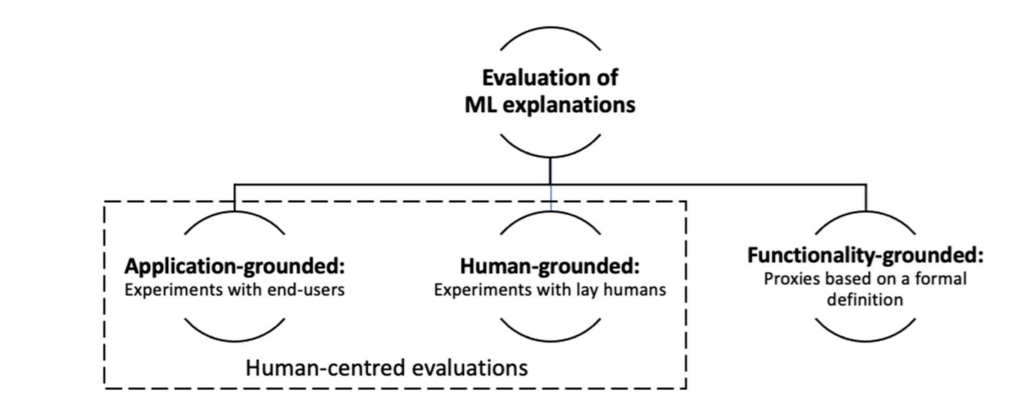
\includegraphics[scale=0.6]{xAI_types}
\caption{groups of explanations \cite{13}}
\label{fig:x cubed graph}
\end{figure}


As the task explored is Handwritten text generation (a task well understood by humans), I chose to focus on the human-grounded methods - methods that are measured by their quality and their human interpertablity, in contrast to methods measured by the scores of a specific matrix.

